\documentclass[../../master_thesis_np.tex]{subfiles}
\graphicspath{{./imgs/}}

\begin{document}
	\chapter{Analysis of Structure and Dynamics}
	Simulations of ABPs ensembles offer an interesting possibility: they make it possible to investigate the physical systems without the limitations that an experimental setup would have. In simulations it is possible to work in a case with the same number of agents every time, keeping the physical conditions fixed, without all non-idealities, having computational power and time as the only limitation. This is crucial to study statistical properties of a system that displays fascinating behaviors.
	
	\section{Methods}
	Our investigation in structure and dynamics is based upon a small, but hopefully complete, set of tools that help unveiling how particles place themselves with respect to one another and how do they move {\color{blue} insert citation about 1994 Nobel, "where atoms are, what atoms do"}.
	
		\subsection{Pair Correlation Function}
		Pair correlation function, \emph{radial distribution function}, or simply $g(r)$ describes the variation of density with respect to distance to a reference in a system; it is a function only of the separation $r_{12} = \abs{\vb{r}_1 - \vb{r}_2}$ between any pair of particles. It quantifies how particle in an ensemble position one with respect to each other, giving information about the \emph{structure} of the system. This function plays a key role in physics of matter since it is possible to measure it in radiation-scattering experiments and it is often used in cases where, differently from our problem, particles' positions are not directly accessible.
		
		It is possible to derive definitions for $g(r)$ starting from first principles, like phase-space distribution functions, as it is done in \cite{hansen90a}. Here we will use the Dirac's $\delta$-based expression, since it the most useful in cases where particle's positions are known,
		\begin{equation}
			\left\langle \frac{1}{N} \sum_{i=1}^{N} \sum_{j=1}^{N}{}' \delta (\mathbf{r} - \mathbf{r}_j + \mathbf{r}_i) \right\rangle = \rho g(r)
		\end{equation}
		where the prime on the summation sign means not counting terms with $i = j$. It is possible to show that the left hand side approaches the value of the overall number density $\rho$ at large distance.
		
		In order to compute $g(r)$ in our simulations, we first need to take distances between all pairs of particles (counting twice the same couple) accounting for periodic boundary conditions as any particle became the center of the system, similarly to the periodic interaction method in section \ref{intrange}. Then, to simulate the behavior of a sum of deltas, we divide simulation space in bins by radius, where the area of each bin is computed as the intersection between a circular crown and a square, to respect the geometry of our simulation box without introducing biases. Now we just normalize by the number of particles and the density to make $g(r) \to 1$ at long distance.
		
		\subsection{Polarization}
		Whenever the agents of a system have a preferred axis, as is the case for ABPs, it becomes worthwhile to analyze their nematic order, i.e.\ the order in the orientation degree of freedom of agents. This is useful especially when particles have non symmetric (in some axis) shape. Our particles are assumed to be perfectly symmetrical circles (spheres in 3D), but still, the presence of a well defined swimming direction introduces a relevant anisotropy in the system. 
		
		For global polarization, we use the following definition
		\begin{equation}
			P = \frac{1}{N} \abs{\sum_{k=1}^{N} e^{i \theta_k(t)}} 
		\end{equation}
		where $\theta_k$ is the orientation of $k$-th particle. This parameter is $1$ when all particles directions are aligned and $0$ when all particles are pointing in different directions. 
		
		\subsection{Cluster Size Distribution}
		As discussed in section \ref{literature}, ensembles of ABPs tend to cluster when an attractive interaction is present or conditions (velocity, packing fraction) are right for MIPS to occur. In most cases, system clusters as a whole, leaving at most some particles in a gaseous phase outside of the cluster. Observing the evolution of such systems, nonetheless, it is possible to observe long periods of time during which ABPs are only partially clustered, moving in small groups across the simulation boards. 
		
		It is possible to extract some information about partial clusters from the $g(r)$, but, being originally created to study systems a whole, it is not the optimal tool. In order to get some insight about partial clustering, which often happens as a transient state before global clustering, we developed the cluster size distribution. 
		
		Our method was built using DBSCAN, a density-based clustering algorithm, which was originally created for data-science but, with the right parameters, can become useful for physics. DBSCAN starts from a point and adds to the cluster associated with that point all the others which are at a distance of less than a threshold. A point having more than $Mp$ points in its vicinity is said \emph{core point} or \emph{seed}. A point in the vicinity of a \emph{core point} is a \emph{border point}. All the others are \emph{noise points}. Using $1$ as $Mp$ (i.e.\ a cluster must be formed with at least 2 points) and particle radius or interactions range as threshold distance, this algorithm's results correspond to the common sense conception of what a cluster is. The advantage of adapting an existing algorithm is that it has some very fast pre-built implementations which are probably more efficient than one could write from scratch.
		
		Getting cluster sizes as the result of a DBSCAN passage, it becomes easy to compute the sample cluster size distribution function, that is, plotting sizes on a histogram.
		\subsection{Local Polarization}
		As explained in previous section, local properties are useful to observe, in particular in transients. When aligning interactions are present and packing fraction is small or we are in a transient, small clusters of particles tend to align their directions, so that measuring the global polarization $P$ would get in the same result of a disordered system, close to $0$. We can exploit the fact that clustering algorithms assign points to clusters and then measure how polarized the single groups are, meaning we compute a local polarization order parameter. Averaging over clusters, this parameter $\bar{P}$ will be close to $1$ even if $P$ is kept low by the different orientations of clusters, making it a good parameter to study local properties and short range interactions.
		
		\section{Coulomb Flocking as a Phase Transition}
		As mentioned in section \ref{literature}, \citeauthor{martin-gomez_collective_2018}, as well as \citeauthor{negi_emergent_2022} showed how inserting an explicitly aligning interaction in the simulation can make the whole system polarize, meaning all particles move in the same direction. This phenomenon is called \emph{flocking}.
		
		Here, we show how a repulsive off centered interaction, although with limited range, can lead an ABPs system to reach a flocking state. The selected interaction force is $F(r) = kr^{-2}$, akin to a Coulomb or gravitational force, where $k$ is a constant. When both the off center magnitude $\alpha$ and the constant $k$ have a positive value, front sides of interacting particles repel each other, meaning that two particle swimming towards each other will tend to align their orientations. Here we stress the fact that when all particles in ensemble have the same velocity and clustering is not present, a head-to-head collision is by far the most frequent, and for sure a head-to-tail collision is almost impossible, since two particles with the same directions will chase each other without ever touching.
		
		\begin{figure}[htp]
			\centering
			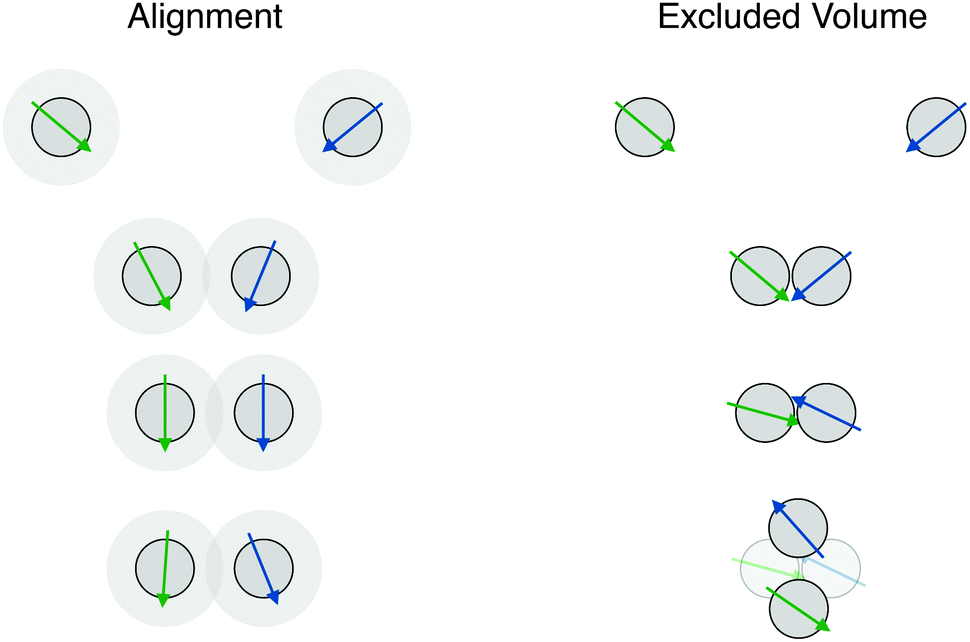
\includegraphics[width=\textwidth]{alignment.png}
			\caption{Behavior of two particles with aligning interactions, compared with excluded volume steric interaction only \citeauthor{martin-gomez_collective_2018}.}
			\label{fig:alignment}
		\end{figure}
		
		In Figure \ref{fig:alignment}, an example of how the alignment process works. Differently from our case, the interaction in mentioned work is an explicitly aligning torque where $T \sim \sin( \theta_{i}-\theta_{j} )$, where particles orientation are \emph{explicitly} included in the expression and $\abs{T}$ has a clear minimum where $\theta_{i} = \theta_{j}$. Our alignment comes automatically from applying a force to a non centered position. 
		
		In Figure \ref{fig:flock40}, an example of how flocking transition happens with $k = 10$, with an interaction range of $40 \mu \text{m}$.
		\begin{figure}[htp]
			\centering
			\subfloat[][]{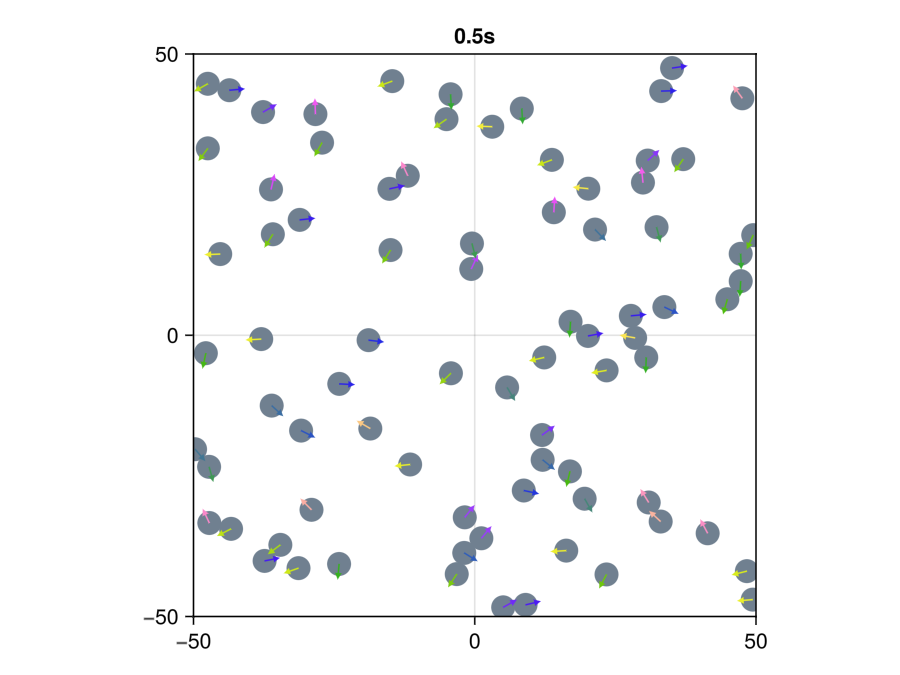
\includegraphics[width=.3\textwidth]{coulombrange40/situation0.5s.png}}
			\subfloat[][]{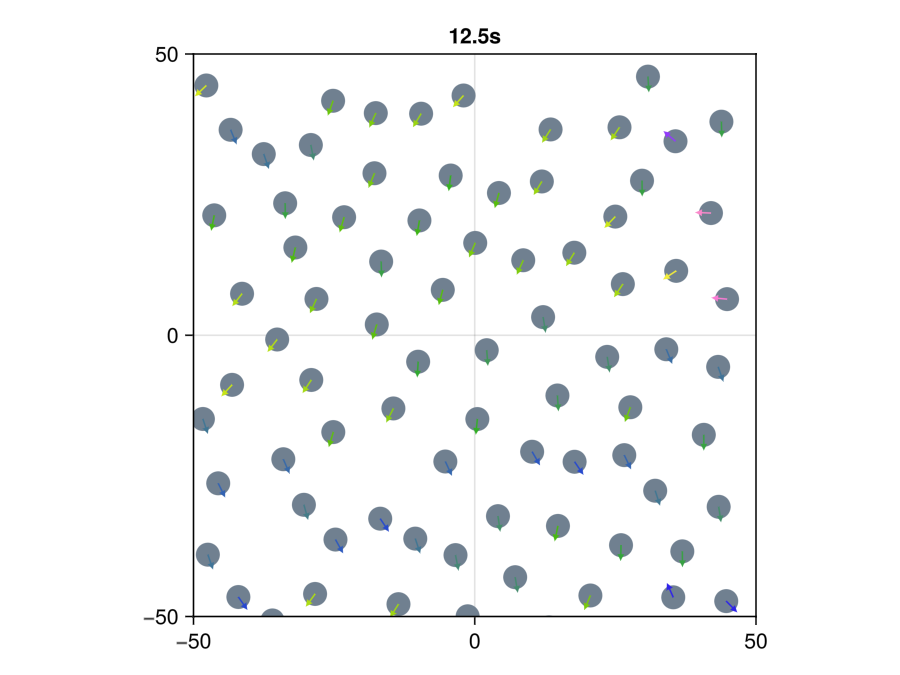
\includegraphics[width=.3\textwidth]{coulombrange40/situation12.5s.png}}
			\subfloat[][]{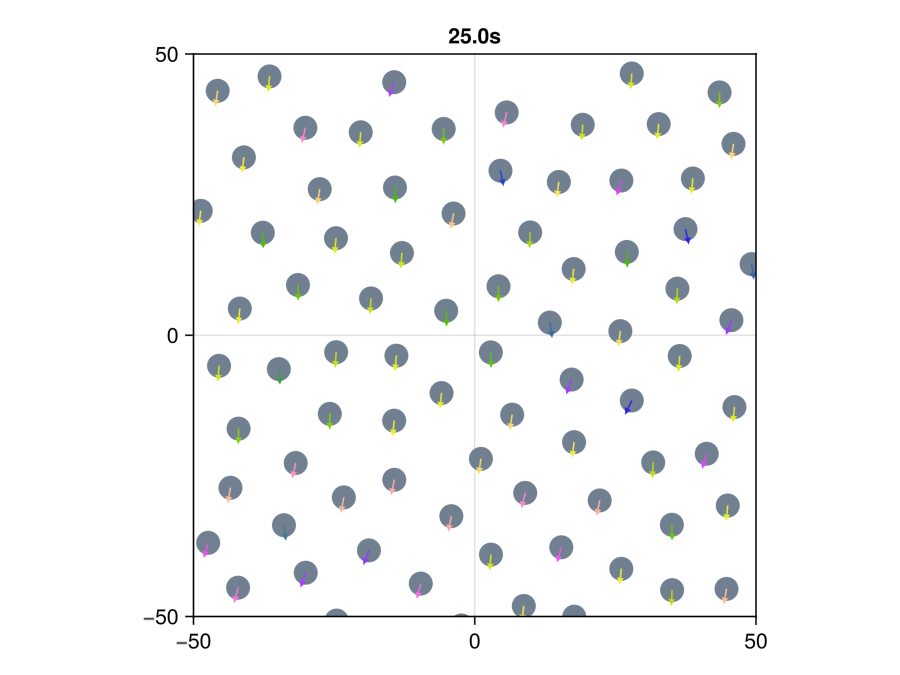
\includegraphics[width=.3\textwidth]{coulombrange40/situation25.0s.png}}\\
			\subfloat[][]{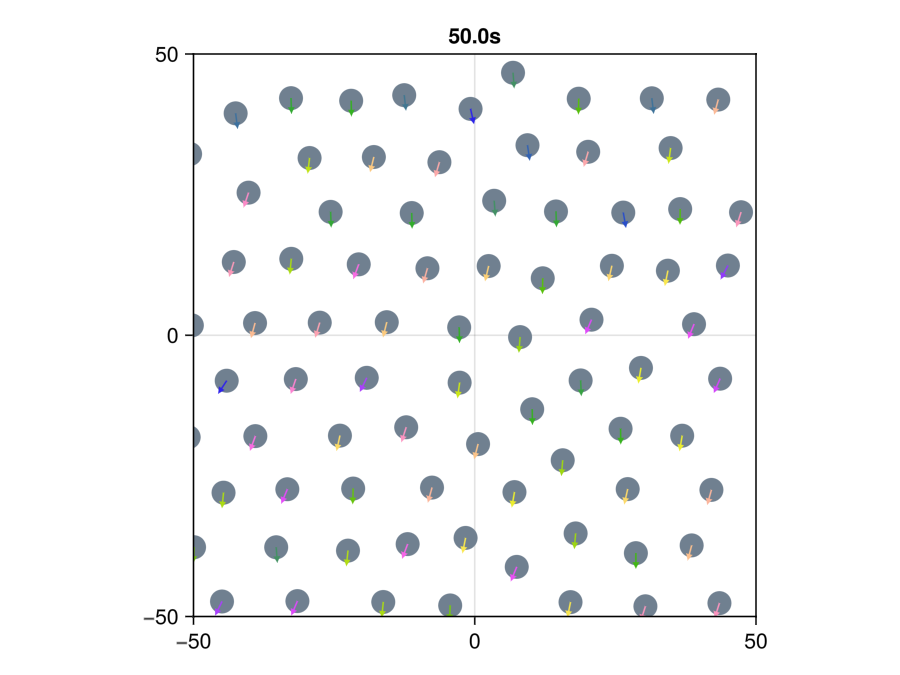
\includegraphics[width=.3\textwidth]{coulombrange40/situation50.0s.png}}
			\subfloat[][]{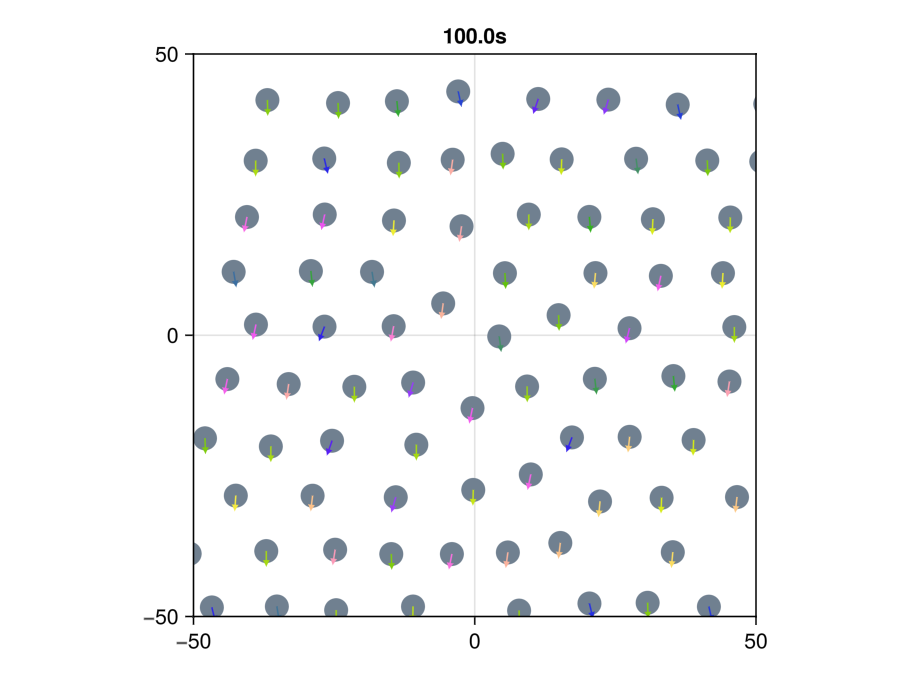
\includegraphics[width=.3\textwidth]{coulombrange40/situation100.0s.png}}
			
			\caption{\textbf{NOT DEFINITIVE} Flocking transition: all particles in the system tend to polarize after few seconds. }
			\label{fig:flock40}
		\end{figure}
			
		We studied flocking as a II order phase transition, using the global polarization $P$ as order parameter and varying $\alpha$, to change the magnitude of orientations coupling. The range of interaction is $5 \mu \text{m}$, which, being $2.5R$, with $R$ particle radius, is enough to make particles interact only with one layer of particles around them, simulating a nearest-neighbor interaction. Though interactions range is so short, a long-range order establishes for large enough $\alpha$, making the whole ensemble polarize.
		
		As a result, Figure \ref{fig:phasetrans} shows the expected behavior of a II order phase transition: as the order parameter $P$ gets with a discontinuity from 0 to 1, its susceptibility diverges to a peak when $\alpha$ approaches critical value and then returns back close to zero (see, as a reference, Figure \ref{fig:martin_flocking3}).
		
		\begin{figure}[htp]
			\centering
			\subfloat[][]{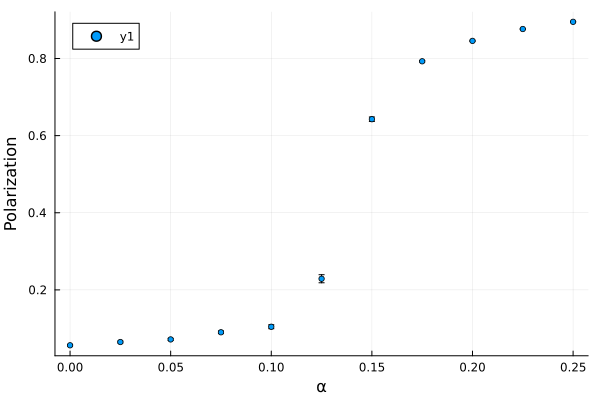
\includegraphics[width= \subfigwidth]{phasetrans/polar.png}}\\
			\subfloat[][]{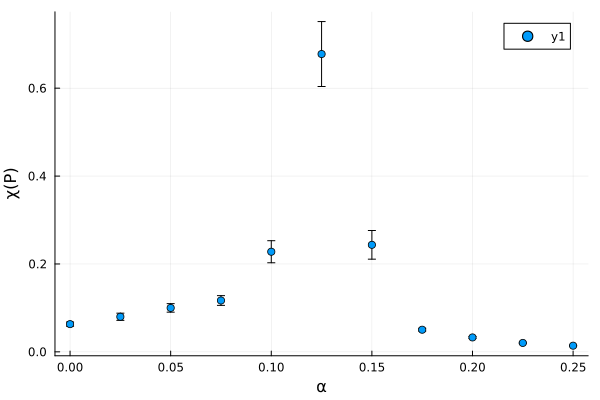
\includegraphics[width= \subfigwidth]{phasetrans/suscpolar.png}}			
			\caption{\textbf{NOT DEFINITIVE} Diagrams for polarization and relative susceptivity for the transition to ordered phase.}
			\label{fig:phasetrans}
		\end{figure}
		
		\section{Aligning Lennard Jones: Clustering and Local Order}
		Lennard Jones (LJ) is the potential which has the best chance of representing well real world dynamics (see section \ref{qualitative}), so it is worthwhile to study it in detail, to see how it affects individual and collective behaviors of ABPs ensembles. In order to do that, we investigated both global and local polarization, as well as clustering, to better understand the effects of the different model parameters on both positional and orientational degrees of freedom.
		
		\subsection{Velocity}
		In order to study the effect of velocity, we first computed all the quantities of interest in the case of passive particles with an aligning LJ interaction, and then added a self propulsion velocity. An active speed makes the system non-isotropic, giving a preferred direction to particles, so we also investigated how velocity interacts with the sign of the directional coupling parameter $\alpha$, repeating the analysis for positive and negative values of it.
		
		The interaction used is LJ with parameters $\sigma = 2R$, with $R$ particle's radius, and strength parameter $\epsilon \sigma = 0.1 J$. Magnitude of $\alpha$ is kept fixed at $0.5$, changing the sign. Simulations involved $250$ particles in a square of $175 \mu\text{m}$ side, for a resulting packing fraction of $\sim 0.1$. Simulation time is 1000 s. 
		
		\begin{figure}[htp]
			\centering
			\subfloat[][]{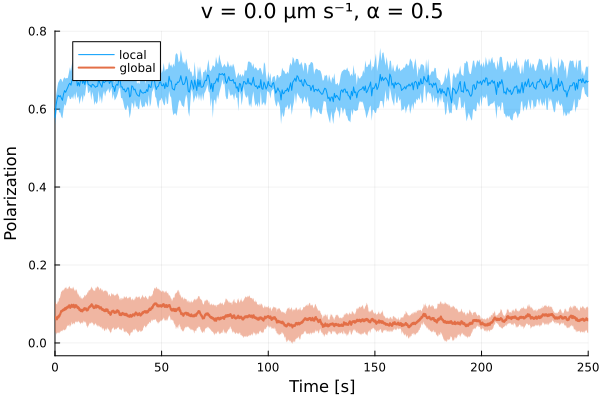
\includegraphics[width=.3\textwidth]{lj_velocity/polar_oc0.5_v0.0.png}}
			\subfloat[][]{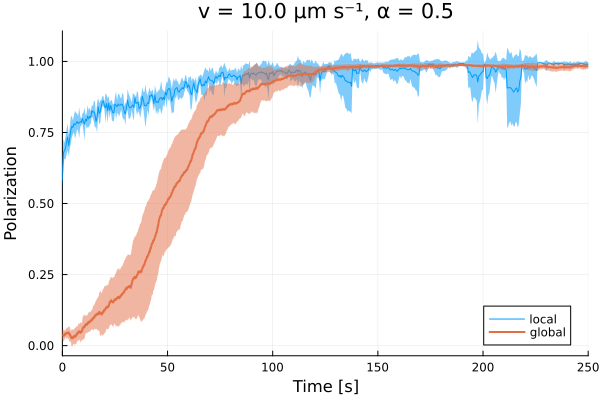
\includegraphics[width=.3\textwidth]{lj_velocity/polar_oc0.5_v10.0.png}}
			\subfloat[][]{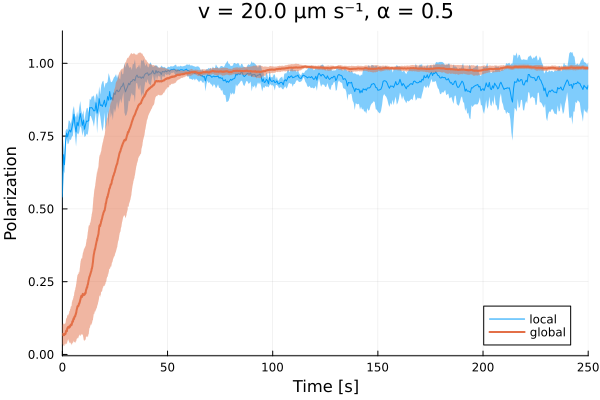
\includegraphics[width=.3\textwidth]{lj_velocity/polar_oc0.5_v20.0.png}}\\
			\subfloat[][]{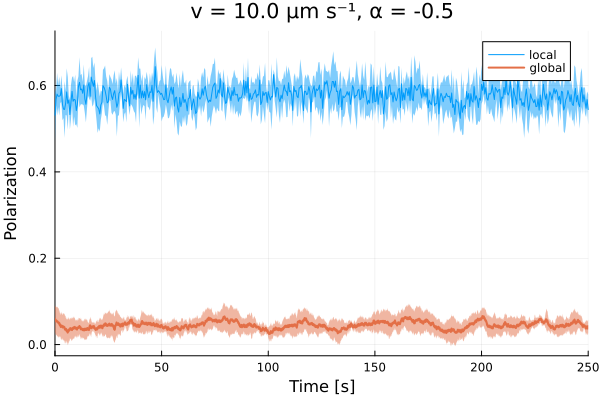
\includegraphics[width=.3\textwidth]{lj_velocity/polar_oc-0.5_v10.0.png}}
			\subfloat[][]{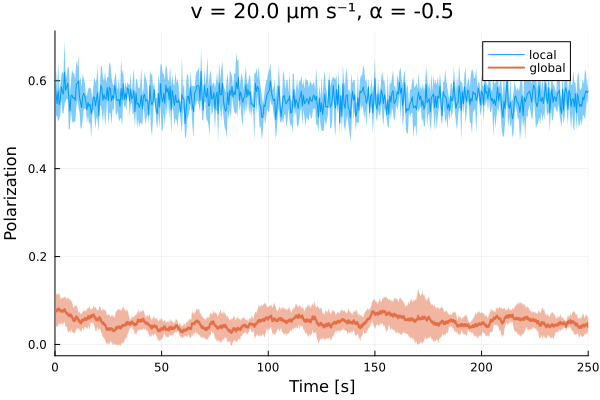
\includegraphics[width=.3\textwidth]{lj_velocity/polar_oc-0.5_v20.0.png}}
			
			\caption{\textbf{NOT DEFINITIVE}  Average of 5 simulations, strip around line is stddeviation}
			\label{fig:lj_velocity_pol}
		\end{figure}
		
		In Figure \ref{fig:lj_velocity_pol} it is noticeable how an ensemble of passive particles with an aligning interaction has a baseline local polarization, while the global is almost zero. Adding self-propulsion has the consequence of making the system polarize, with a transient length that depends on the velocity: faster particles tend to align faster. A noteworthy characteristic is that particles with interacting position on the back do not tend to align at all.
		
		This can also be noticed in Figures \ref{fig:lj_velocity_situation} and \ref{fig:lj_velocity_cluster}, where, when the off center position is on the back, velocity tends to hinder clustering, leading to a more sparse final situation. This can be due to the aforementioned fact about velocity: all particles have the same velocity so a head-to-tail collision is unlikely, as a consequence the off cen
		
		\begin{figure}[htp]
			\centering
			\subfloat[][]{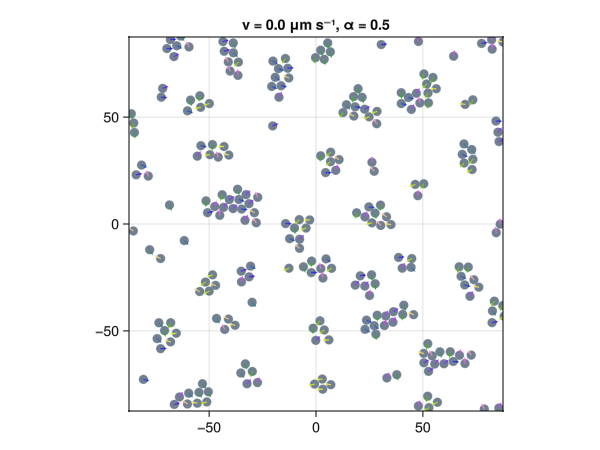
\includegraphics[width=.5\textwidth]{lj_velocity/situation_oc0.5_v0.0.png}}
			\subfloat[][]{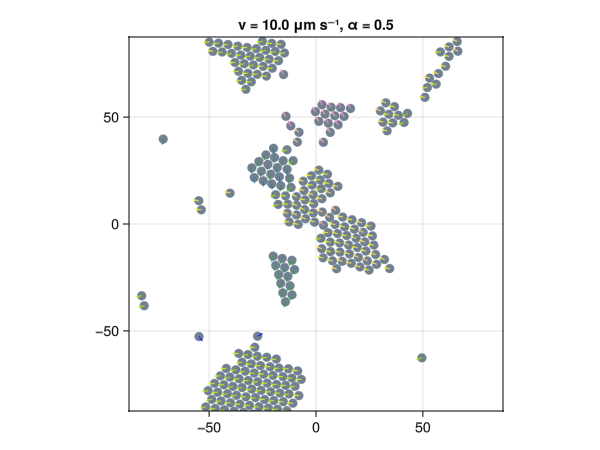
\includegraphics[width=.5\textwidth]{lj_velocity/situation_oc0.5_v10.0.png}}\\
			\subfloat[][]{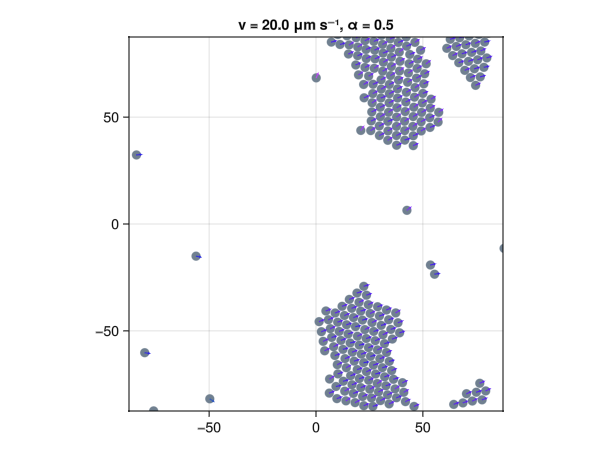
\includegraphics[width=.5\textwidth]{lj_velocity/situation_oc0.5_v20.0.png}}
			\subfloat[][]{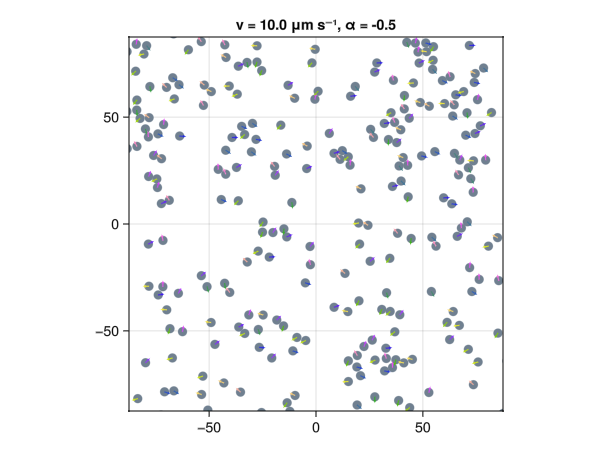
\includegraphics[width=.5\textwidth]{lj_velocity/situation_oc-0.5_v10.0.png}}\\
			\subfloat[][]{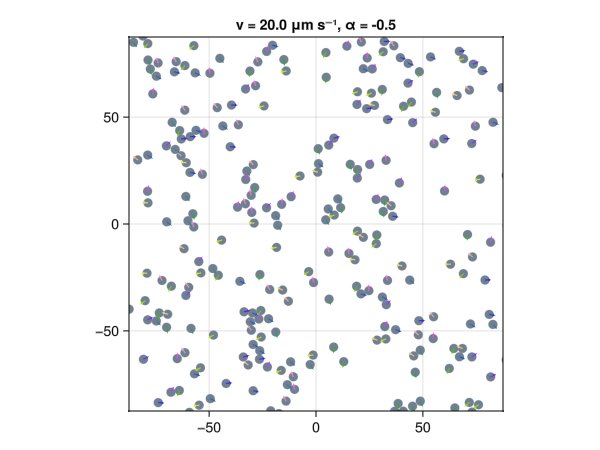
\includegraphics[width=.5\textwidth]{lj_velocity/situation_oc-0.5_v20.0.png}}
			
			\caption{\textbf{NOT DEFINITIVE}  }
			\label{fig:lj_velocity_situation}
		\end{figure}
		
		
		\begin{figure}[htp]
			\centering
			\subfloat[][]{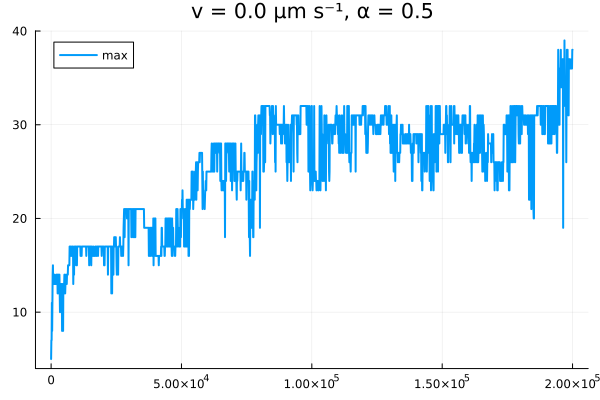
\includegraphics[width=.5\textwidth]{lj_velocity/cluster_oc0.5_v0.0.png}}
			\subfloat[][]{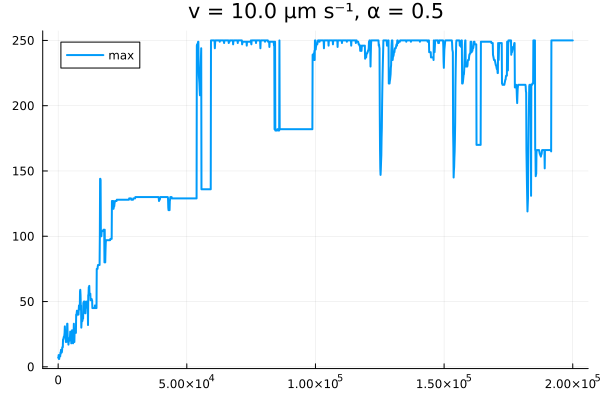
\includegraphics[width=.5\textwidth]{lj_velocity/cluster_oc0.5_v10.0.png}}\\
			\subfloat[][]{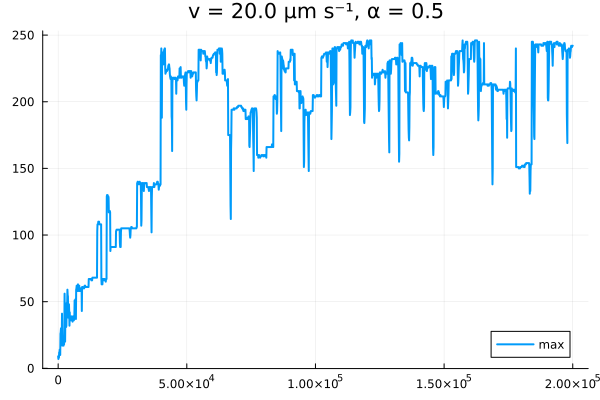
\includegraphics[width=.5\textwidth]{lj_velocity/cluster_oc0.5_v20.0.png}}
			\subfloat[][]{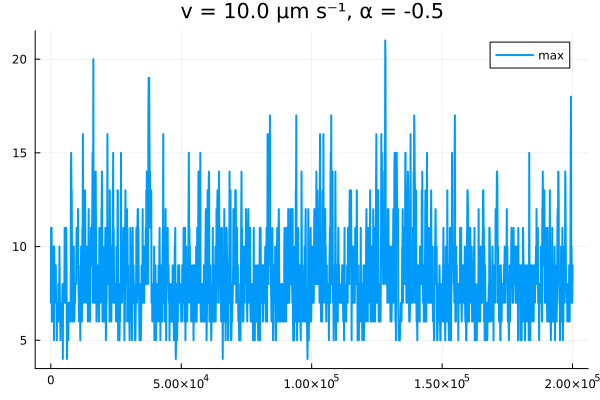
\includegraphics[width=.5\textwidth]{lj_velocity/cluster_oc-0.5_v10.0.png}}\\
			\subfloat[][]{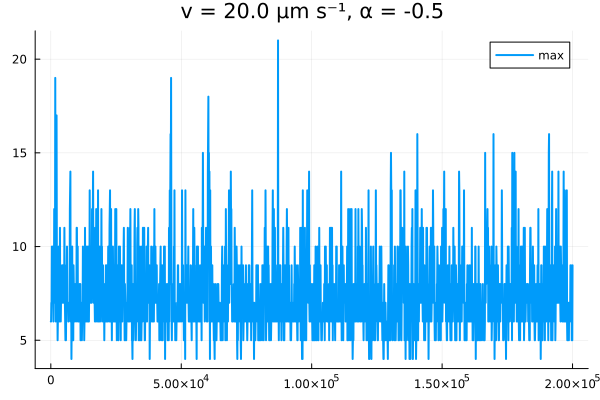
\includegraphics[width=.5\textwidth]{lj_velocity/cluster_oc-0.5_v20.0.png}}
			
			\caption{\textbf{NOT DEFINITIVE}  }
			\label{fig:lj_velocity_cluster}
		\end{figure}
		
		\begin{comment}		
		\subsection{Velocity Distribution}
		\subsection{Angular Velocity}
		\subsection{Orientation Coupling}
		\subsection{LJ strength $\epsilon$}			
		\end{comment}
	
	\subsection{Velocity Distribution}
	\subsection{Angular Velocity}
	%\subsection{Radius}??????
	
		

\end{document}